\documentclass[a4paper]{article}
\usepackage{geometry}
\usepackage{multicol}
\usepackage{minted}
\usepackage{amsmath, dsfont, mathtools, amssymb}
\usepackage{fontspec}
\usepackage{xcolor}
\usepackage{wrapfig}
\usepackage{graphicx}
\usepackage{enumitem}

\pagestyle{empty}
\geometry{top=0.5cm, bottom=0.5cm, left=0.5cm, right=0.5cm} 

\setlength{\columnsep}{1pt} % Remove space between columns


% Redefine section commands to use less space
\makeatletter
\renewcommand{\section}{\@startsection{section}{1}{0mm}%
                                {-1ex plus -.5ex minus -.2ex}%
                                {0.5ex plus .2ex}%x
                                {\normalfont\large\bfseries}}
\renewcommand{\subsection}{\@startsection{subsection}{2}{0mm}%
                                {-1explus -.5ex minus -.2ex}%
                                {0.5ex plus .2ex}%
                                {\normalfont\normalsize\bfseries}}
\renewcommand{\subsubsection}{\@startsection{subsubsection}{3}{0mm}%
                                {-1ex plus -.5ex minus -.2ex}%
                                {1ex plus .2ex}%
                                {\normalfont\small\bfseries}}
\makeatother

% Don't print section numbers
\setcounter{secnumdepth}{0}
\setlength{\parindent}{0em}
\setlength{\parskip}{0.2em}
\setlist[enumerate]{noitemsep, topsep=0pt, leftmargin=*}
\setlist[itemize]{noitemsep, topsep=0pt, leftmargin=*}
\newcommand{\mathcolorbox}[2]{\colorbox{#1}{$\displaystyle #2$}}


\begin{document}

\small

\begin{multicols*}{3}
    \section{Cost and benefit}
    $ES=TB-TC$; $WTP\in B$; $OC(n_1) = C(n_1) + TB(n_2)$; $MB(n) = TB(n)-TB(n-1) = \frac{dTB}{dn}$; $NM = MB - MC$

    \begin{itemize}
        \item Continue doing / at n units: $NM \geq 0$
        \item Choose one over another: $ES(n_1) \geq ES(n_2)$
        \item Consume n units of either good: $NM=NM$
        \item Consume n units of goods by cost table: marignal cost table $\to$ trace lowest to highest
    \end{itemize}

    Willing to do for free / sunk cost $\to$ ignore.

    \tiny

    In allocation of fixed amount of resources, a rational individual should always allocate the additional unit of resources to the activities with the highest \textbf{marginal} benefit.

    \normalsize

    \section{Trading and advantage}

    ABS adv.: c of prod. < c of prod. of another producer; ABS adv. and comp. adv. is \textbf{mutually exclusive}

    "n y per x" $\implies y = nx$;

    comp. adv. if $OC$ of good is \textbf{lower} than another producer; $\textcolor{red}{OC_{A}} = \frac{\textcolor{red}{C_A}}{\textcolor{blue}{C_B}} = \frac{\textcolor{blue}{U_B}}{\textcolor{red}{U_A}}$ ($\textcolor{blue}{B}$ per $\textcolor{red}{A}$)

    Optimal outcome when producer specialize good with comp. adv.; Specialization gain $\propto$ $OC_{A} - OC_{B}$; Specialize at comp. adv.

    admissible $TOT \in \{\min{OC_{A}}, \max{OC_{B}}\}$; Best for specializing $\textcolor{red}{A}$ is the $\textcolor{red}{OC_A}$ of producer of $\textcolor{blue}{B}$

    Curve: plot quantity of $A-B$; PPC: Highest producable lvl of goods market; CPC: Highest consumable lvl of goods market; $PPC: \textcolor{red}{A} = \textcolor{blue}{(-OC_B)B}+c$

    "\$a A, \$b B" $\implies bA=aB$;

    Multiple producer $PPC$: connect ends from lowest to highest slope (shift $\textcolor{red}{A}$ up if $\textcolor{red}{OC_A}<\textcolor{blue}{OC_B}$)

    Economy: Closed $CPC=PPC$, Open $CPC > PPC$ as consume imported and produced

    \begin{itemize}
        \item Consumption constraint ratio $r=A:B$, plot $A=rB$ find intersection with $PPC$
        \item Consumption constraint ratio $r$ and table
        \item Multiple points $(A,B)$, world price of goods, producer selected one point: find range of $TOT$: 1. compute income at each point 2. $I_p > I_{`p}$
    \end{itemize}

    2-pt line: $y=\frac{y_2-y_1}{x_2-x_1}(x-x_1)+y_1$;

    \section{Demand and supply}
    Perfect comp. market: Take price given, d\&s determines market price

    Curves plot $P-Q$; D curve down slope: $P\uparrow$ buyer no buy as much, can switch to alts; S curve up slope: $P\uparrow$ producers sell more; The demand curve of an inferior good can be upward sloping.

    Market d/s: $Q_m = Q_1 + Q_2 + \ldots$ (change subject to $Q$); \textbf{Find kink point(s)}; \textcolor{orange}{Demand}: take \textbf{highest} curve; \textcolor{magenta}{Supply}: take \textbf{lowest} curve

    Equilibrium: market clears; Producer surplus: area underneath $P=\$p$ and above $S$; Consumer surplus: area above $P=\$p$ and below $D$;

    Price change \textbf{DOES NOT LEAD TO} demand / supply change, only \textbf{QUANTITY} demanded / supplied.

    \begin{minipage}{\linewidth}
        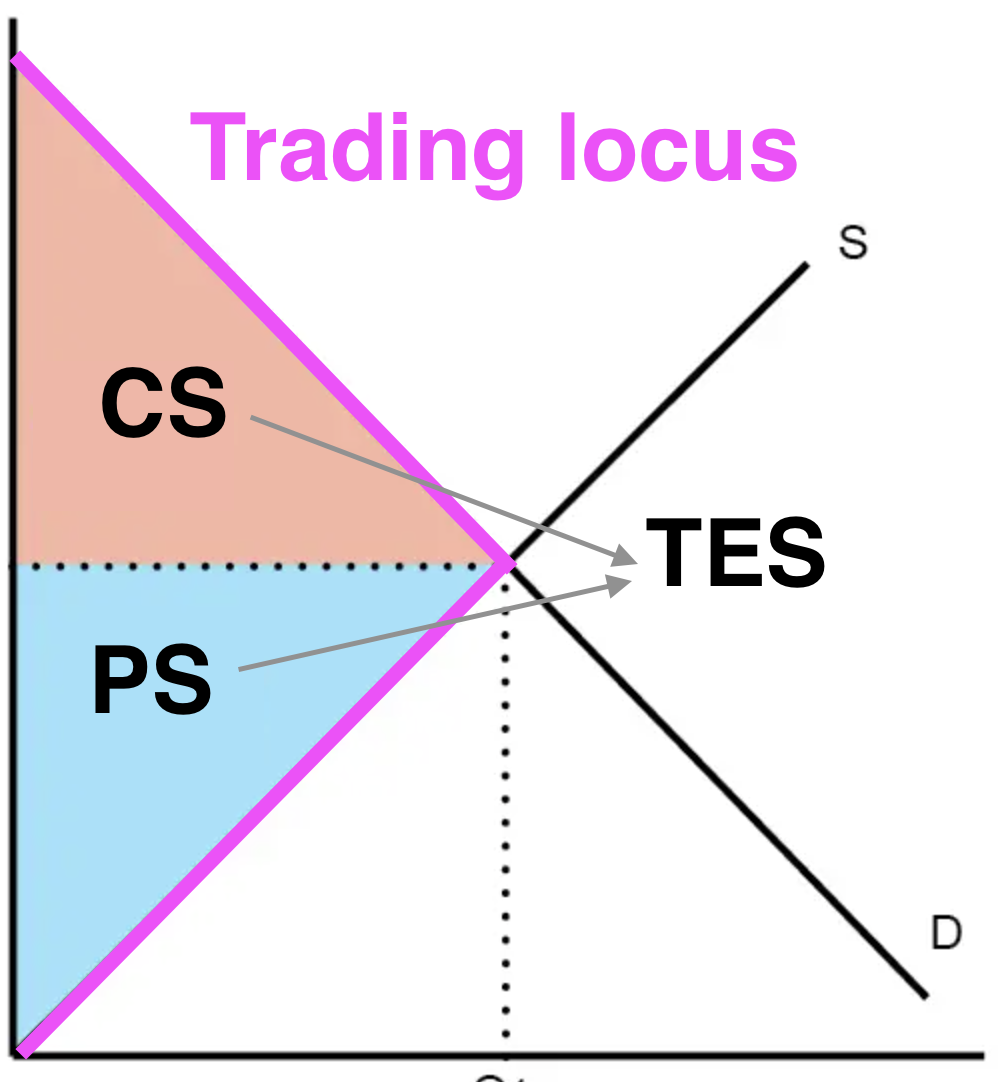
\includegraphics[width=0.48\linewidth]{./csps.png}
        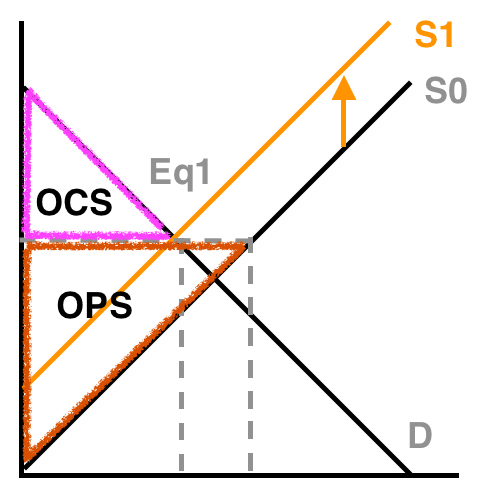
\includegraphics[width=0.48\linewidth]{./csps2.jpg}
    \end{minipage}

    Surplus $P > P^*, \textcolor{magenta}{Q_s} > \textcolor{orange}{Q_d}$; Shortage $P < P^*, \textcolor{magenta}{Q_s} < \textcolor{orange}{Q_d}$; $TES$ maximized at eq.; d/s curves shifts to right if increase.

    Quantity excess = $|\textcolor{magenta}{Q_s} - \textcolor{orange}{Q_d}|$;

    \begin{minipage}{\linewidth}
        \begin{tabular}{l|l|l}
            Type     & $\textcolor{orange}{Q_d}$ : $I \uparrow$ & $\textcolor{orange}{\eta_{d,I}}$ \\
            \hline
            Normal   & $\uparrow$                               & $>0$                             \\
            Luxury   & $\uparrow$                               & $>1$                             \\
            Inferior & $\downarrow$                             & $<0$                             \\
        \end{tabular}
    \end{minipage}

    \begin{minipage}{\linewidth}
        \begin{tabular}{l|l|l}
            Type of good B & $\textcolor{orange}{Q_{d,A}}$ : $P_B \uparrow$ & $\textcolor{orange}{\eta_{d,\text{cross}}}$ \\
            \hline
            Substitute     & $\uparrow$                                     & $>0$                                        \\
            Complements    & $\downarrow$                                   & $<0$                                        \\
        \end{tabular}
    \end{minipage}

    \begin{itemize}
        \item Limited \textcolor{magenta}{n supply}: $\textcolor{magenta}{Q=n}$ curve, CS: intersect with D, \textbf{PS: intersect with S}
        \item Raised money purchase $R$: $\textcolor{magenta}{Q}=\frac{R}{P}$ curve
        \item Supply at price is negative: return 0
        \item Price guarantee: $P=\$p$, $Q=|\textcolor{magenta}{Q_s} - \textcolor{orange}{Q_d}|$;
    \end{itemize}

    \tiny

    Calc prog 1: Area of polygon; Enter number by number for each vertex corrdinates \textbf{in order}

    Calc prog 2: 2 simu. eq.; Enter $ax+by=c$ for each equation. First $b$ must not be 0

    \normalsize

    \section{Comparative statics}

    \tiny

    Factor ; Demand shift ; Example

    | Population ; $\uparrow, \rightarrow$ ; Number of ppl and water demand |

    | Income to normal goods ; $\uparrow, \rightarrow$ ; Income and restaurant demand |

    | Income to inferior goods ; $\downarrow, \leftarrow$ ; Income and instant noodle demand |

    | Price of substitutes ; $\uparrow, \rightarrow$ ; If electric car is expensive, ppl will buy more petrol cars |

    | Price of complements ; $\downarrow, \leftarrow$ ; If petrol is cheap, ppl will buy more petrol cars |

    | Expectation of future price ; $\uparrow, \rightarrow$ ; If ppl expect price of house to rise, they will buy more now |

    | Taste ; $\uparrow, \rightarrow$ ; If apple has recently been found to be healthy, ppl will buy more apples |

    \normalsize

    \section{Elasticity}
    Base $\eta=\frac{\%\Delta Q}{\%\Delta P}$; 2-pt $\eta = \frac{Q_1-Q_0}{Q1+Q_0}\cdot\frac{P_1+P_0}{P_1-P_0}$; line-pt $\eta = \frac{P}{Q}\cdot\frac{1}{\text{slope}}=-\frac{PQ_x}{QP_y}$; revenue $=PQ$; maximized \textbf{at mid-point} of demand curve

    $\textcolor{orange}{\eta_d}$: $<-1$ elastic, $=-1$ unit elastic, $>-1$ inelastic, $=0$ perfectly inelastic, $=-\infty$ perfectly elastic; $\textcolor{magenta}{\eta_s}$: $<1$ elastic, $=1$ unit elastic, $>1$ inelastic;

    Const: $\ln Q = a + b\ln P \to \eta=b$ @ all pts.; Only pay \$$m \to \eta = -1$; Supply y-intercept $P_s=m\textcolor{magenta}{Q_s}+c, c$ $>0\to\textcolor{magenta}{\eta_s}>1$, $=0\to\textcolor{magenta}{\eta_s}=1$,$<0\to\textcolor{magenta}{\eta_s}<1$

    $\textcolor{orange}{\eta_I} = \frac{I}{\textcolor{orange}{Q}}\cdot\frac{\textcolor{orange}{dQ}}{dI}$; $\textcolor{orange}{\eta_{cross}} = \frac{P_B}{\textcolor{orange}{Q_A}}\cdot\frac{\textcolor{orange}{dQ_A}}{dP_B}$;

    $\textcolor{orange}{Q_1}=a-\frac{\Delta \textcolor{orange}{Q}}{\Delta P}P_1+\frac{\Delta \textcolor{orange}{Q_1}}{\Delta P_2}P_2-\frac{\Delta \textcolor{orange}{Q}}{\Delta I}I$;

    $\uparrow\%\Delta P = \frac{\textcolor{orange}{\%\Delta Q_d}}{|\textcolor{orange}{\eta_d}|+\textcolor{magenta}{\eta_s}}= -\frac{\textcolor{magenta}{\%\Delta Q_s}}{|\textcolor{orange}{\eta_d}|+\textcolor{magenta}{\eta_s}}$; $\uparrow\%\Delta Q = \textcolor{magenta}{\eta_s}\times\%\Delta P$;

        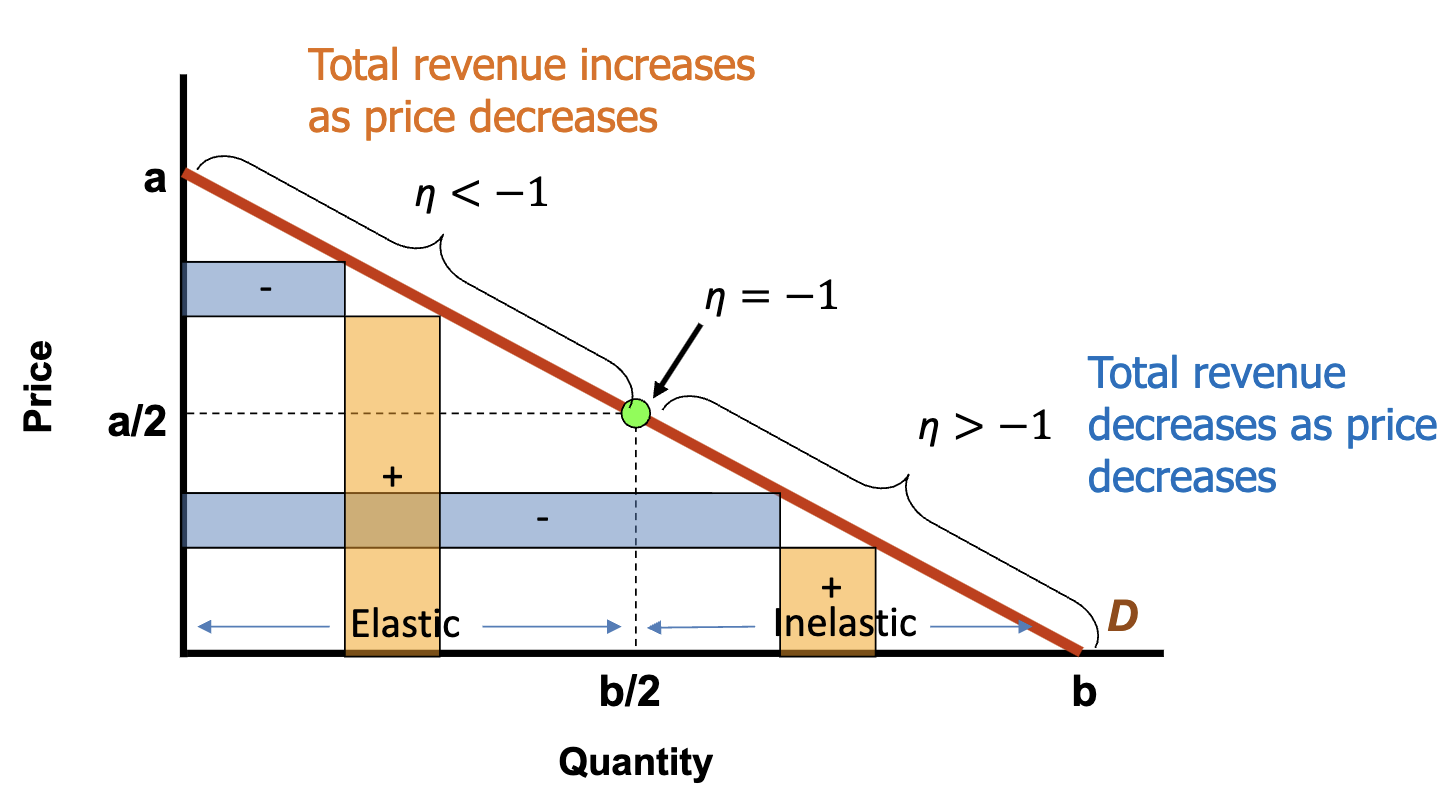
\includegraphics[width=\linewidth]{./total-revenue.png}

        Price elasticity of demand ($\textcolor{orange}{-\eta_d}$) $\propto$ \textbf{substitutes} / time to adjust (find subs.) / specifity of classification / luxurious nature / price point;

    $\textcolor{magenta}{\eta_s}\propto$ difficulity of producing more / time to increase supply / availability of inputs / specifity of geographic scope

        \section{Taxes and subsidy}

    $ts=s-t$; $\textcolor{orange}{D}$ shift vertically $ts$, $\textcolor{magenta}{S}$ shift vertically $-ts$ (shift by add to $P$); Wedge: $Q=Qe$ (shifted equilibrium); $P_P$ intersection $\textcolor{magenta}{S}$ with wedge, $P_C$ intersection $\textcolor{orange}{D}$ with wedge; $|ts|=P_P-P_C$; $|ts|\times \textcolor{magenta}{Q^*}=\text{gov tax revenue}$;

        Consumer per-unit share burden $|P_C-P^*|$; Producer per-unit share burden $|P_S-P^*|$; Less elastic side more burden / benefit

        DWL: The lost economic surplus when the socially optimal quantity of a good is not produced $\propto$ elasticity (imagine scissors) ($\propto \eta_s, \frac{1}{\eta_d}$)


    \begin{itemize}
        \item Given required DWL / cost: \textbf{Shift demand} by $ts$ -> re-subject to $P$, \textbf{equalize with S} to find $Q$ -> DWL / cost formula
    \end{itemize}
    \begin{minipage}{\linewidth}
        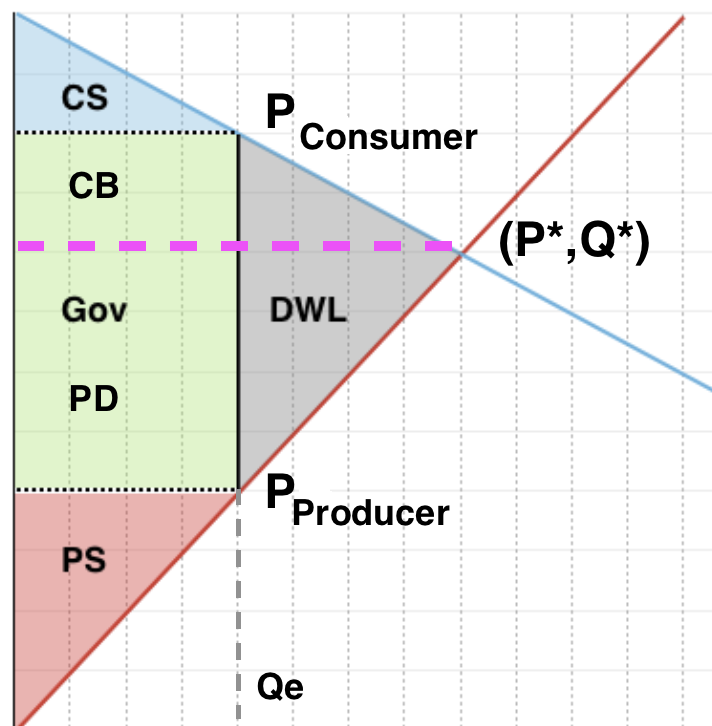
\includegraphics[width=.48\linewidth]{./tax.png}
        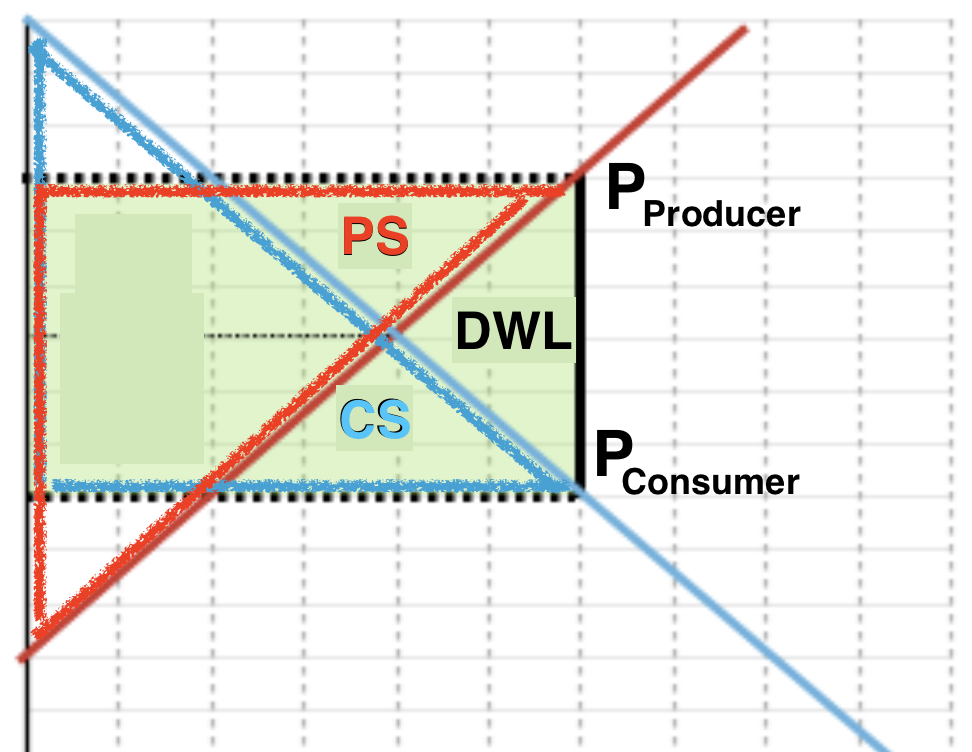
\includegraphics[width=.48\linewidth]{./tax2.png}
    \end{minipage}

    \tiny

    \section{[SOLS] Cost and Benefit}

    "Summer vacation; Normally work 40 hours a week, \$12 per hour; Parents paying \$1500 for cabin; You have to pay \$200 for food; Usually pay \$300 rent, \$75 food; Travel cost to vacation \$50; Your opportunity cost for vacation"

    Ignore: \$1500 cabin (not by you), \$300 rent (had to be paid anyway), total cost of food to go on vacation \$$200-75$

        \rule{1\linewidth}{0.4pt}

        "Given table columns [Quantity, consumer1, consumer2...,], cells willingness to pay, consider the market demand curve, the marginal willingness to pay for the 5-th good is:"

        Iterate from largest number for 5 times.

        \rule{1\linewidth}{0.4pt}

        "Given table columns [Time, worker1, worker2], cells cost for working time, allocate to minimize cost and have total of 6 hours of output"

        Convert to marginal benefit table, trace from lowest to highest for 6 iterations. Return count.

        "Allocate to have maximized total economic surplus for hourly benefit of \$123"

        Give marginal benefit table index from smallest to largest. Calculate $ES(n)$ at a random index, then surrounding index. Find peak $ES$ and return traced count at that index.

        \rule{1\linewidth}{0.4pt}

        "MB for consuming coffee: $MB=229-20n$. Cost for one cup of coffee = 35. The total economic surplus for consuming coffee is:"

        Will only consume if $MB(n) \geq MC(n)$: $229-20n \geq 35$; $n \leq 9.7$; $ES(n) = TB(n) - TC(n)$; $TB(n) = 229n - 10n^2$; $TC(n) = 35n$; $ES(9.7) = TB(9.7) - TC(9.7)$

        \rule{1\linewidth}{0.4pt}

        "Per month of watching n movies: $MB(n)=660-14n$; Upon paying a monthly subscription fee of 19 dollars, Calvin will be eligible to watch any movie at P dollars per movie. If Calvin decides to watch 27 movies per month under the scheme, then we can infer that the price per movie (P) is less than or equal to X dollars and more than Y dollars."

        Given $MC(n) = P$, each decision must satisfy $MB(n) \geq MC(n)$: $MB(27) \geq P$; $MB(27) = 660 - 14 \cdot 27 = 282$; $MC(n) = P$; $P < MB(28)$; $MB(28) = 660 - 14 \cdot 28 = 268$; Therefore, $X = 282$ and $Y = 268$.

        \section{[SOLS] Trading and advantage}

        B: $D = 21 − 7F$; S: $D = 144 - 8F$; "Consume 16 units of F, consume how much D?"


    $OC_{F,B}=7, OC_{F,S}=8$; $OC_{F,B} < OC_{F,S}$ $\implies$ B specialize F, S specialize D; B makes 3 F, so S makes $16-3=13$ D; $D=(144-8(16-3))$

        "Admissable world TOT (in F per D)"; $\in \{\frac{1}{8}, \frac{1}{7}\}$;

        "Trade with world F@\$9.5 D@\$1, consume 16 units of F, consume how much D?"; $TOT_F=9.5, TOT_F>OC_{F,S},OC_{F,B}$ so both make F (comp. adv. against world): $D_S=\frac{144}{8}=18>16 \implies 2 + \frac{21}{7} = 5$: profit of 5 F gives $5\times9.5$ D.

        \rule{1\linewidth}{0.4pt}

        "Alison can produce 123 kgs of bread or 123 kgs of cupcakes per week. Philip can produce 51 kgs of bread or X (X < 51) kgs of cupcakes per week. They decide their time allocation together. Suppose their joint preference dictates that the bread consumption to cupcake consumption ratio must be 3:1. "

        Find individual PPC curve -> market PPC -> intersect with $B=3C (\frac{B}{C}=\frac31)$ -> find $C$ and $B$

        \rule{1\linewidth}{0.4pt}

        "Karis and Oni are the only farmers in Islandia, a small island nation. Karis can harvest 5 bananas or 20 pineapples per day. Oni can harvest 20 bananas or 5 pineapples per day. Islandia is currently a closed economy, i.e., no trade with the rest of the world. Islandians like to consume bananas and pineapples at 2 to 1 ratio (ratio of 2 bananas and 1 pineapple) per day. How many bananas would Karis produce?"

        Find individual PPC curve -> market PPC -> intersect with $B=2P$ -> find $B$ -> specialization: $OC_{O,B} < OC_{K,B}$; O can produce 20 bananas, so Karis will produce $P-20$ bananas.

        \rule{1\linewidth}{0.4pt}

        "Cindy and Veronica constitute a small economy that produces only two goods: tea and cakes. We know that Cindy has the comparative advantage in producing tea and Veronica has the comparative advantage in producing cakes. If they fully specialize in the production that they have comparative advantage in, they will produce a total of 102 kgs of tea and 71 kgs of cakes per week."

        "(a) If the admissible range for terms of trade is between 0.5 kgs of tea per kg of cakes and 3 kgs of tea per kg of cakes, we can infer that Cindy can produce \textbf{A1} kgs of cakes per week and Veronica can produce \textbf{A2} kgs of tea per week."

        T/week, C/week;

        | C (Tea)   | a             | A1             |

        | V (Cake)| A2             | b             |

        Because C specializes in Tea, and V specializes in Cake, a=102, b=71.

        We know $OC_{C,\text{Cake}} > OC_{V,\text{Cake}}$ by given speicalization.

        Admissible TOT $\in \{OC_{C,\text{Tea}}, OC_{V,\text{Tea}}\}$.

        TOT $\in \{3, 0.5\}$ (Tea per Cake); $OC_{C,\text{Cake}} = \frac{a}{A1} = 3$; $A1 = \frac{102}{3} = \underline{\mathbf{34}}$; $OC_{V,\text{Tea}} = \frac{A2}{b} = 0.5$; $A2 = 71\times0.5 = \underline{\mathbf{35.5}}$

        "(b) Continue from the previous question. Suppose this small economy opens up its trade with the rest of the world. The world prices are \$1 per kg of tea and \$X per kg of cakes. If both Cindy and Veronica will specialize in the production of tea only, we may infer that X is \textbf{A3}: smaller / larger than \textbf{A4}."

        World Tea per Cake $= \frac{X}{1} = X$. (Tea per Cake gives $OC_\text{Cake}$)

        For them to produce tea only: $OC_{W,\text{Cake}} <\min\{OC_{C,\text{Cake}}, OC_{V,\text{Cake}}\}$; $OC_{W,\text{Cake}} <0.5$; $X \underline{\mathbf{<0.5}}$

        "(c) Continue from the previous two questions. Suppose the world price of tea remains \$1 per kg but the price of cakes is \$2 per kg. If Cindy and Veronica together decide to consume tea and cakes at the ratio of 1.7:1 (i.e., for each 1 kg of cakes, they would want to consume 1.7 kgs of tea), they will consume \textbf{A5} kgs of tea and \textbf{A6} kgs of cakes per week."

        Given $X=2$, specialization is the same as provided by question.

        Total value of production: $102 \times 1 + 71 \times 2 = 244$; Consumption ratio: $1.7C = T$; Consumption: $T + 2C = 244$; $T + 2\frac{T}{1.7} = 244$; $T = \underline{\mathbf{112.11}}$; $C = \frac{244-112.11}{2} = \underline{\mathbf{65.95}}$

        \section{[SOLS] Demand and supply}

        "D: $P=93-53Q$, S: $P=63$; $Eq= (0.57, 63)$. Government raises \$$126$ dollars to buy goods back from the market. After government enters market, on new demand curve, when price is 126 dollars, $Q_d$ is?"

        Government demand: $Q=\frac{126}{P}$; $Q(126) = 1$;

        "Market equilibrium quantity? Quantity of good left in market?"

        Original demand (rearrange) $Q=\frac{93-P}{53}$; $Q_d=Q+Q_g$ -> Intersect with supply $P=63$ -> $Q^*$; Quantity left $Q^* - \frac{126}{63}$;

        \rule{1\linewidth}{0.4pt}

        "Give table columns [Quantity, supplier n (\$)...], cells are marginal cost for each quantity. Marginal cost for providing $n$-th unit of good:"

        Iterate from smallest to largest for $n$-th unit.

        \rule{1\linewidth}{0.4pt}

        "Given table columns [Quantity, buyer n (\$)], cells are marginal WTP for each quantity. What is marginal buyer's WTP when quantity is $n$:"

        Iterate from largest to smallest for $n$-th unit.

        \rule{1\linewidth}{0.4pt}

        "$S_1: P=20+4Q, S_2: P=10+Q, D: P = 45 - 1.5Q$; Welfare loss if restricted quantity at $50\%$ of market equilibrium?"

        Change $S$ terms $P \to Q$, find $Q_m=Q_1+1_2$ -> find intersect (\textbf{kink points}) $Q_m,Q_1$ and $Q_m,Q_2$ -> identify intersection curve with $D$ -> find equilibrium $Q^*$ -> find intersects of $Q=Q^*\times 0.5$ with $D$ and market supply curve (identify intersection curve) -> area of polygon (4 points)

        \section{[SOLS] Comparative statics}

        Event 1: The number of university fresh graduates emigrating out from Utopia has been increasing.
        Event 2: The Utopian government decides to hire more university fresh graduates in Utopia.

        We can predict increase in the equilibrium salary of university fresh graduates and uncertain change in the equilibrium level of employment for university fresh graduates.

        \rule{1\linewidth}{0.4pt}

        "For country A: D: $Q = 22.4-1.5P$; S: $Q=2P-16.57$"; Country A is considering opening up its milk market to its neighbouring country B for a year. If the market is opened up, Country B is expected to buy 1 million boxes per year from country A at any price. New equilibrium price? Surplus of local group?"

        Shift D by $D_B: Q_B=Q_A+1$ -> Intersection $D_B$ with S

        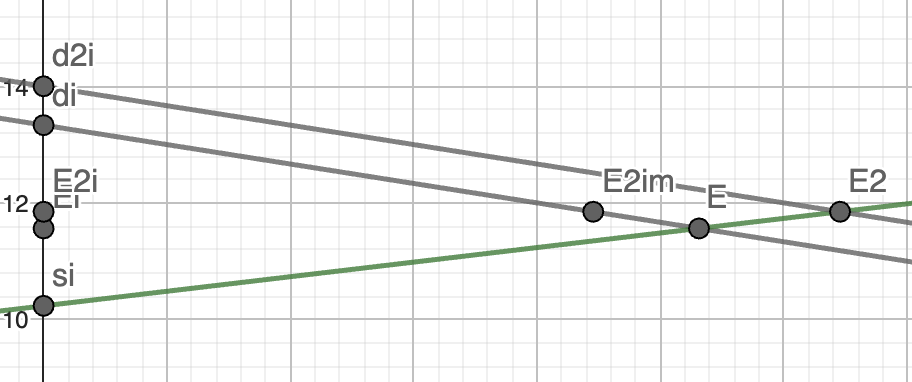
\includegraphics[width=\linewidth]{./i2.png}

        OCS: Area(di,E2i,E2im), OPS: Area(E2i,E2,si)

        "How will the local consumers and producers as seperate groups react to the opening of the milk market to country B?"

        Cosumer willing to spend up to $|OCS-CS|$ to lobby the government ($OCS < CS$ ? against : for) opening.
        Producer willing to spend up to $|OPS-PS|$ to lobby the government ($OPS < PS$ ? against : for) opening.

        "To make two group happy, can tax by:"

        Tax ((Producer for) ? Producer : Consumer) amount $\in \{|OCS-CS|, |OPS-PS|\}$ and give to ((Producer for) ? Consumer : Producer).

        \section{[SOLS] Elasticity}

        “Titanic” in cinemas is \textbf{less price elastic} than "Titanic" online, as online has more substitutes.

        \rule{1\linewidth}{0.4pt}

    $Q_x=10-3P_x+2P_y-0.7I$; Good X is an \textbf{inferior} good as $I\uparrow Q_x\downarrow$, Good Y is a \textbf{substitude} as $\frac{\Delta Q_A}{\Delta P_B} = 2 > 0$.

        \rule{1\linewidth}{0.4pt}

        The CEO of a restaurant chain group said, “For each 1 percent price hike, we lose 5 percent of our diners.”; All of the following are not conclusions:

        (I) demand is price inelastic.

        (II) a price increase will increase total revenue.

        (III) the price elasticity of demand is -0.5.

        (IV) demand for dining will go up as price decreases.

        \rule{1\linewidth}{0.4pt}

        If a downward shift of the demand curve leads to a 5\% decrease in equilibrium price and a 10\% decrease in equilibrium quantity, the price elasticity of \textbf{supply} is $\frac{10}{5} = 2$.

        \section{[SOLS] Taxes and subsidy}

        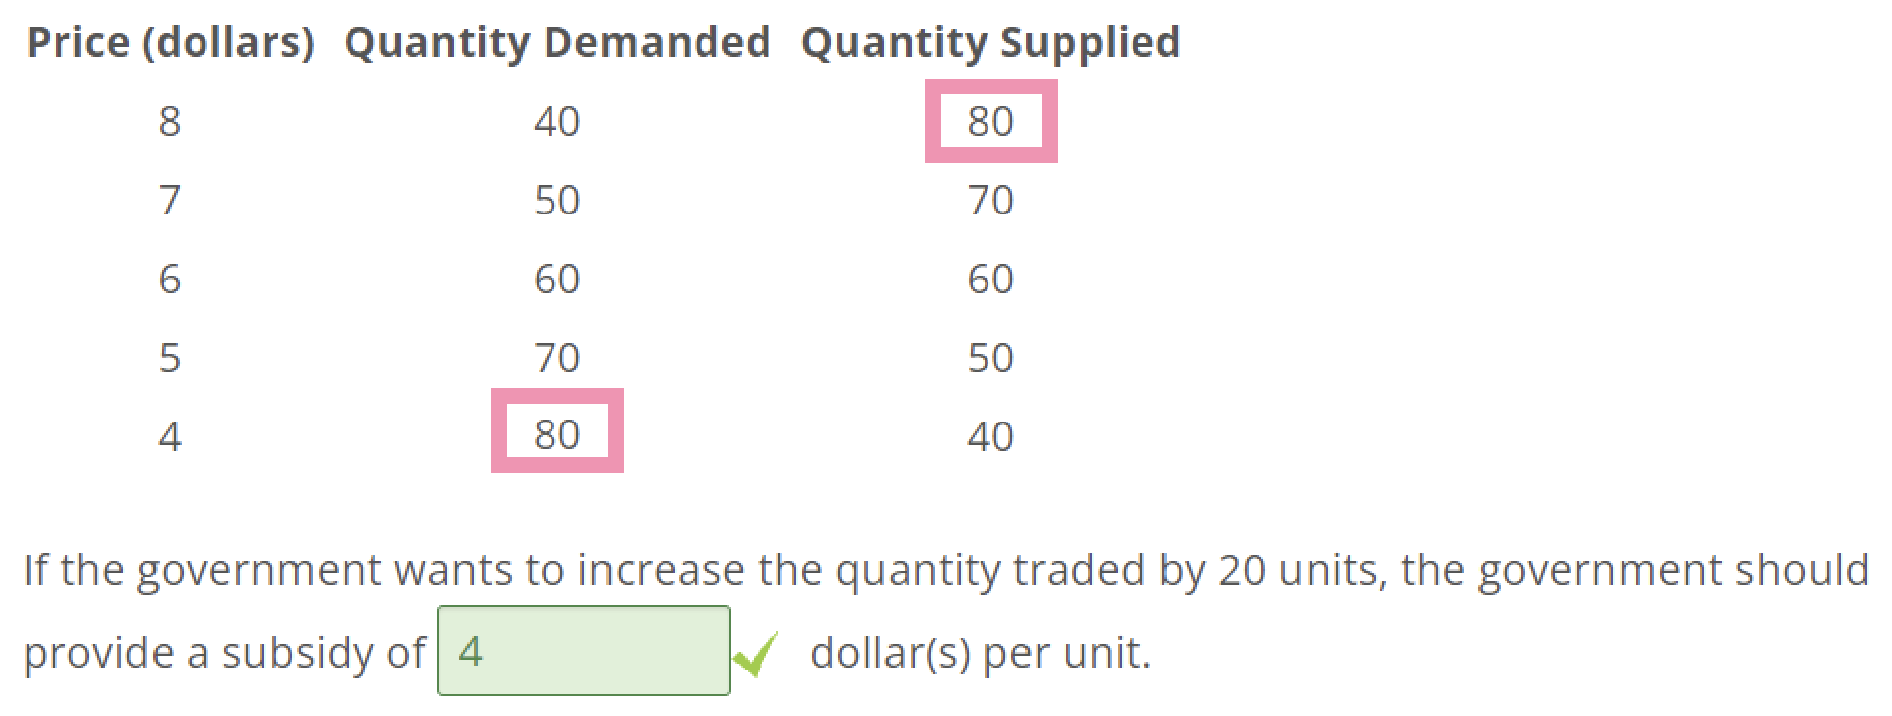
\includegraphics[width=\linewidth]{./tax3.png}

        \rule{1\linewidth}{0.4pt}

        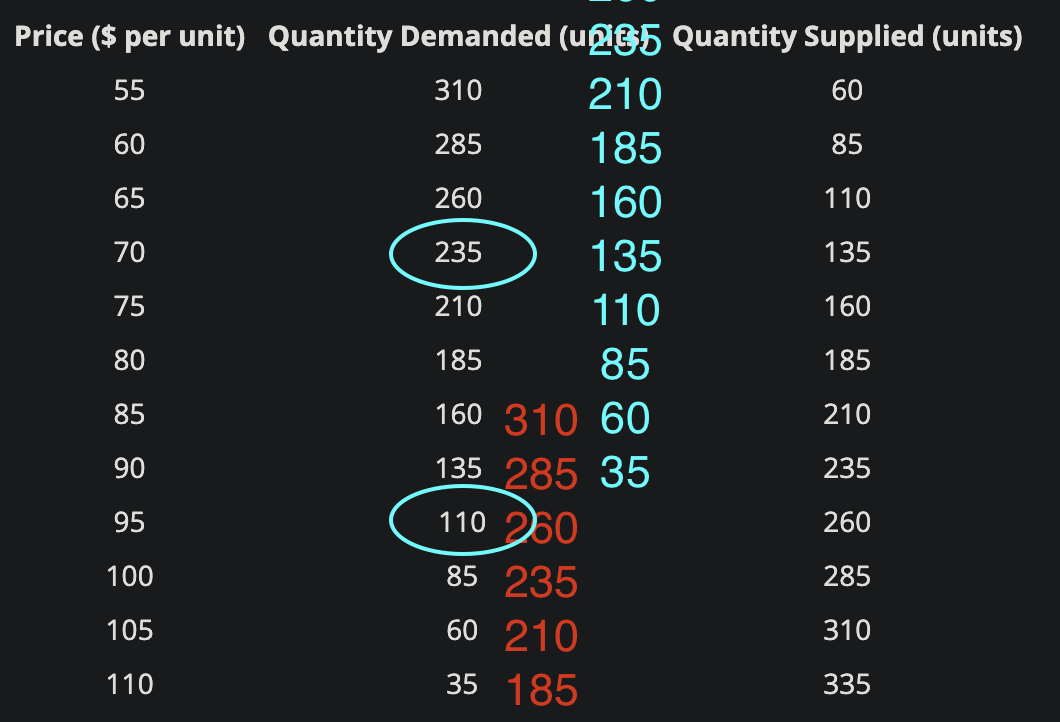
\includegraphics[width=\linewidth]{./ts-table.png}

        Suppose initially the chocolate market is in an unregulated equilibrium. If the government imposes a tax of \$30 for each unit of the chocolate sold, the new equilibrium price paid by the consumers will be 95.

        Given the above information, the government’s tax revenue will be \$3300

        Suppose initially the chocolate market is in an unregulated equilibrium. If the government imposes a subsidy of \$20 for each unit of the chocolate sold, the new equilibrium quantity would be 235 units.

        \rule{1\linewidth}{0.4pt}

        D: $Q=230-2P$; S: $Q=3P-18"$; $Eq = (130.8,49.6)"$; "Price guarantee at \$67 per unit, for when there is insufficient demand. Store the purchased at \$10 per kg. How much quantity brought from guarantee? Producer surplus and guarantee cost?"

        Plot $P=67$ -> intersection with D and S -> $Q=|Q_s-Q_d|$;

        Producer surplus: area under $P=67$ and above $S$. Cost: $Q \times 67 + Q \times 10$;

        "Switch to subsidy policy, how much subsidy needed for 67 per kg? PS and cost?"

        Plot $P=67$ -> intersection with S -> $x=Q_s$ -> intersection with D find $P_d$ -> $ts = P_s - P_d$

        Producer surplus: same, Cost: $|ts| \times Q_s$;

        \rule{1\linewidth}{0.4pt}

        "D: $Q=590-P$; S: $2.5P-230$; $Eq = (355.71,234.29)$; To reduce the consumer price by 35\%, the subsidy to impose is? The TES will rise by?"

    $P_d = 234.29 \times (1-.35)$; $Q=590-P_d \to Q= 2.5P_s-230 \implies P_s$; $|ts| = P_s - P_d$;

        TES rised is $Q\times |ts| - \frac{|ts| \times (Q-Q^*)}{2}$

        "Suppose impose budget 54000, what is max subsidy?"

        Shift demand (rearrange to subject $P$): $D: P=590-Q+|ts|, S: P=\frac{Q+230}{2.5}$ -> equalize, rearrange to subject Q. \textbf{Subsitute to government expense formula} $54000 = |ts| \times Q \to$ solve for $|ts$ with quad equation.

\end{multicols*}
\end{document}